\documentclass{article}

 \usepackage[utf8]{inputenc} %Stationær ÆØÅ
%\usepackage[ansinew]{inputenc} %Bærbar ÆØÅ?

%\usepackage{url} % Allows hyperlinks
\usepackage[hyphens]{url} %URLs
\usepackage{graphicx} % Allows figures
\usepackage{etoolbox} %for configuration of sloppy
\usepackage{tabularx}
%Section style
\usepackage{xcolor}

\definecolor{secnum}{RGB}{102,102,102} 

\makeatletter
    \def\@seccntformat#1{\llap{\color{secnum}\csname the#1\endcsname\hskip 16pt}}
\makeatother
%end section style

\apptocmd{\sloppy}{\hbadness 10000\relax}{}{} %adds hbadness to sloppy
\setlength{\paperheight}{297mm} %Sets the page to an A4
\setlength{\paperwidth}{210mm}	%Sets the page to an A4

\begin{document}

\begin{titlepage}
\begin{center}
\textsc{\Large IT Sikkerhed}\\[0.5cm]
\textsc{OPGAVE B: Sikkerhedsanalyse af sociale medier}\\[0.5cm]
\vspace{2 cm}
\begin{tabular}{ll}
Kasper Passov & pvx884\\
\end{tabular}
\end{center}
\vspace{5 cm}
\newpage
\tableofcontents
\end{titlepage}

\section{Resumé af firma og system}
\subsection{Firmaets risiko niveau}
Firmaet BIOmedix er et firma med høj sårbarhed overfor informations tyveri. En lækage af forsknings resultater kan have meget alvorlige konsekvenser for BIOmedix, da salg af disse resultater og patenter der er kommet deraf er deres primære indkomstkilde. Dette betyder IT sikkerheden bør være i firmaets fokus for at beskytte disse aktiver. 

\subsection{Resumé af det nye system}
Der skal indføres fire nye sociale medier i BIOmedix. Dette har jeg valgt at dele op i 2 grupper. 

\paragraph{Eksterne systemer}
Den ene er 3 sider i de sociale netværker Facebook, Twitter og LinkedIn som jeg vil kalde de eksterne systemer, idet pointer med disse er at give firmaet en mulighed for at kommunikere med folk udenfor firmaet. Jeg har valgt at samle disse systemer i en gruppe da jeg mener der er mange ligheder i hvilke trusler og sårbarheder disse systemer bliver udsat for, og derigennem skal sikkerheden i disse systemer håndteres ens. Kodeord og brugernavne til disse kontoer bliver holdt af kommunikationsafdelingen, som står for opdateringer.

\paragraph{Internt system}
Det sidste system, Yammer, er et lukket socialt netværk for alle firmaets ansatte. Systemet lader dem blandt andet opdatere arbejdsstatus og danne projektgrupper. Jeg vil referer til dette netværk som et internt system, da mange af de trusler og sårbarheder Yammer er udsat for ville kunne bruges på lignende systemer i fremtiden.

\subsection{Sikkerhedsmål}

Sikkerheds målet for både de interne og eksterne netværker, er at have beskyttede kontoer og passwords,
samt at have siderne let tilgængelige. 

\section{Aktiver}
\subsection{Eksterne systemer}
Vores vigtigste aktiv i de eksterne systemer er muligheden for at videregive information til den bredere befolkning. 

\subsection{Interne systemer}
Informationen på det interne system Yammer skal beskyttes fra udekommende, da der vil være store mængder af kritisk information på dette netværk. Derudover skal ansatte have nem og hurtig adgang til information, gerne hvor som helst og når som helst.

\subsection{Begrundelse for aktiver}

\paragraph{Spredning af information}
De eksterne systemers primære funktion er at give firmaet en kommunikations kanal til den brede befolkning. Dette kan både være en nyhed om et gennembrud, et opslag til en ny stilling eller general information om firmaet. Denne aktiv skal bruges til at hæve firmaets omdømme og skal beskyttes ved at holde kommunikations linjen åben og så uhindret som mulig.

\paragraph{Internt information}
Yammer kommer til at indeholde hvad de ansatte arbejder på, hvem de arbejder med, forskningsidéer og filer. Et brud på dette netværk vil blotte alt information BIOmedix har, og gøre det muligt for konkurrenter eller patenttrolde at se hvor langt BIOmedix er med et stykke forskning, og muligvis presse en patent frem inden BIOmedix kan færdiggøre sig. 

\paragraph{Ansattes input}
Uden de ansattes adgang til Yammer, vil dette cloud system ikke være sikkerheds risikoen værd. 
Derfor skal det gøres så nemt som muligt for at de ansattes adgang til Yammer ikke bliver 
hindret af sikkerhedsforanstaltninger.  


\section{Trussels aktører}

\paragraph{Konkurrenter}
Konkurrenterne vil have en interesse i den information og forskning BIOmedix laver.
Derfor må de ses som dem der har mest at vinde ved at bryde ind i systemerne og derfor
den største trussel.

\paragraph{Utilfredse ansatte}
En utilfreds ansat kan lække information kritisk for BIOmedix' forskning.

% Derfor er det vigtigt at holde øje og arbejde med ansatte der er ultifredse.

% \paragraph{Ondsindene}


\paragraph{Internet vandaler}
Det er ikke unormalt for nogen hackere at udnytte et sikkerhedshul i et firma
uden et specifikt formål. De gør dette fordi de kan og syntes det er sjovt. Dette
betyder de oftest går efter sider der har kendte sikkerhedshuller.
Den eneste måde at beskytte sig imod denne gruppe, er at holde sig opdateret indenfor de
seneste sikkerhedshuller, og holde sit system så sikkert de ikke gider bruge
energi på at bryde det.\\
Det er også tit denne gruppe der benytter sig af en stor mængde computere
til et koordineret DoS angreb, hvis formål er at nedlægge systemet.

\paragraph{Internet sabotører}
Internet sabotører er betydeligt farligere end vandaler, da de angriber med
et formål. De er tit ude efter et specifikt stykke information eller er 
blevet hyret til at nedlægge systemet i en kritisk periode. De skal i store
træk håndteres på samme måde som vandalerne, men de er betydelig mere stædige
i deres angreb.

\section{Trusler}

\begin{table}[h!]
    \begin{tabular}{l|l|l|l}
        Trussel                                    & Sandsynlighed & Konsekvens & Risiko\\\hline
        Udbyder lækker passwords                   & 1 & 2 & Lav\\
        Malware password lækage                   & 4 & 4 & Ekstrem\\
        Medarbejder lækage                        & 2 & 4 & Høj\\
        For strenge password regler                & 2 & 2 & Lav\\
        Phishing password lækage                  & 3 & 4 & Høj
    \end{tabular}
    \label{tab:Trusler}
    \caption{Sandsynlighed og konsekvens for de forskellige trusler. Tals betydning kan ses på side 505-507 \cite{Bog}, Risiko niveau er fundet ved hjælp af tabel 14.4 på side 508 \cite{Bog}.}
\end{table}

\paragraph{Udbyder lækker passwords}
Hvis en af udbydernes side bliver kompromitteret, risikere BIOmedix alt information
den side er i besiddelse af. Dette behøver ikke kun være brugere og passwords til
den pågældende side, men også kreditkort information hvis det er bundet til
sider som Facebook kunne være i farer.

\paragraph{Medarbejder lækage}
En utilfreds medarbejder kan lække kritisk information til konkurrenter
eller andre interesserede udekommende. Da BIOmedix har en forholdsvis lille
medarbejder gruppe er risikoen for en sådan lækage ikke stor, men konsekvensen
ville være seriøs. Dette er fordi hvis en medarbejder lækker information
vil det være kritisk information.

\paragraph{Yammer konto mistet via phishing}
En ansat får en mail fra en person der siger han er hans chef eller
IT-ansvarlige og skal bruge hans brugernavn og password. Mailen 
indeholder derefter en trussel om at den ansatte mister sit job hvis 
informationen ikke bliver videregivet.\\
En sådan mail vil kunne få mange ansatte til at give sit password fra
sig, hvis de ikke er informeret om denne form for trussel. 
I det interne netværk Yammer vil en kompromittering af en bruger betyde alt tilgængelig information
er blevet delt med angriberen. 
Dette skal ses som et meget seriøst problem da dette tit vil indeholde kritisk information.

\paragraph{Ekstern konto mistet via phishing}
De eksterne netværk har højst et par kritiske brugere, da det fra firmaet kun er 
kommunikationsafdelingen der behøver adgang til siden. Dette betyder dog også
alle kontoer vil være meget kritiske da de alle vil have administratoradgang til
siden. Hvis en af disse kontoer blive kompromitteret kan det have seriøse konsekvenser
for tilliden til firmaet.

\paragraph{For strenge password regler}
Hvis meget strenge sikkerhedsforanstaltninger kommer i brug, kan det betyde
medarbejderne får problemer med at udfører deres arbejde. Et 12 bogstaver langt
password der ugeligt skal ændres og skal indeholde tegn, tal samt store og små
bogstaver, vil give mange ansatte store problemer og kan derigennem nedsætte
produktiviteten unødigt.

\paragraph{Passwords lækket via Malware}
Malware af forskellige art kan blive overført til ansattes computere. Dette malware
kan så opsnappe passwords og brugernavne, og sende det ud til angriberens computer.\\
Dette kan opsnappe både interne og eksterne passwords alt efter hvilken computer der
er inficeret. 

\subsection{Relevante angreb}

\subsubsection{AP's Twitter-konto}

\begin{figure}
  \begin{center}
    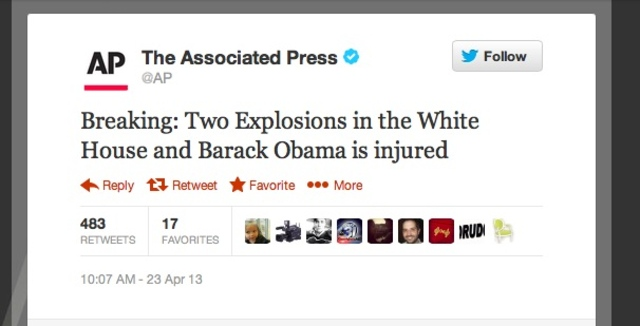
\includegraphics[width=0.6\textwidth]{../Pictures/APTweet.jpg}
  \end{center}
  \caption{Tweeten fra hackeren over nyhedsbureauet Associated Press \cite{APTweetSource}}
  \label{fig:Tweet}
\end{figure}

\paragraph{Angreb}

To af Associated Press' twitter sider blev den 23 april 2013 hacket of en falsk nyhedsmeddeles blev udsendt\cite{TweetStory}. Tweetet kan ses på figur \ref{fig:Tweet}

\paragraph{Relevans for BIOmedix}

Et sådan angreb på BIOmedix kan fjerne tilhængernes tilliden til de eksterne sider. Følgere til siderne
ønsker nyheder fra BIOmedix og ikke misinformation. Derudover kan en sådan hacking lade konkurrenter
samt ondsindede hacker sprede misinformation i BIOmedix navn. 

\subsubsection{LinkedIn password-lækage}

\paragraph{Angreb}
På et forum lagde brugeren "dwdm" 8 millioner krypterede passwords op og bad om hjælp
til at bryde dem. Det viser sig at de 8 millioner passwords blandt andet er fra siden LinkedIn.
Det spekuleres at angriberen allerede havde brudt de en meget stor del af LinkedIn's brugere, da
der var omkring 120 millioner brugere på LinkedIn's side da listen blev frigjort. Dette kan betyde
at "dwdm" allerede havde brudt de svagere passwords, og de 8 millioner var det subset af passwords
han ikke kunne bryde alene\cite{LinkedInStory}.

\paragraph{Relevans for BIOmedix}

Et stort lækage af passwords fra en sådan side kunne betyde alle BIOmedix'
sociale medie sider ville være usikre, hvis det samme password og brugernavn var 
brugt overalt.
Hvis en sådan lækage skete og blev kendt, skal passwordet på den pågældende side, samt
alle sider der benytter det samme password ændres. Derefter skal alt information på
siden tjekkes igennem for ændringer.
Selvom et sådan angreb næppe er gjort af nogen der er interesseret i BIOmedix siden, er
det muligt listen af passwords er blevet solgt til en interesseret konkurent. Derfor kan
det ikke ignoreres selv hvis det ikke er konkurrenter der har lavet angrebet.

\subsubsection{Ex-CIA ansat påstår at have videregivet NSA hemmeligheder} 

\paragraph{Angreb}
En tidligere CIA agent påstår at være kilden til de hemmelige dokumenter der er blevet
lækket til flere nyhedssider. Den lækkede information omhandler et program kaldet PRISM som
den amerikanske efterretningstjeneste bruger til at spionere på privat personer\cite{CIAStory}.

\paragraph{Relevans for BIOmedix}
En utilfreds ansat ville kunne videregive fortrigelig information. Et eksempel kunne være
forskning BIOmedix er i gang med. Denne information kunne være interessant for konkurrenter, da det ville
give dem muligheden for at forske i det samme, og potentielt tage en patent eller udgive resultater
inden BIOmedix er klar til det.

\section{Sårbarheder}

\paragraph{Ansattes password styrke}
Hvis de ansatte får lov til selv at vælge passwords, vil de glemsomme 
tit vælge svage passwords, der vil være genbrugt over mange sider.
Derudover er der flere måder hvorpå en ansats password kan falde i de
forkerte hænder, som phishing og lækager fra netværkssiderne.
% Hvis et password bliver kompromitteret vil  

\paragraph{Kritisk information er ikke på firmastyret servere}
Da Yammer kommer til at indeholde store mængder af kritisk information,
kan det blive et problem for BIOmedix at de ikke har kontrol over
sikkerheden af den information. De er afhængige af Yammer's 
sikkerhedsprotokoller og kan ikke selv indføre nye foranstaltninger hvis
BIOmedix mener det er nødvendigt.

\paragraph{En bruger på alle tre sider}
Hvis den samme bruger bliver brugt på alle tre sider, vil det betyde
at et mistet password vil kræve en gennemgang på alle tre sider. Dette
gælder også for passwords som "BIOmedixFacebook" og "BIOmedixLinkedIn" 
som værende ens.

\paragraph{En konto til eksterne sider}
Da der kun er en konto til de eksterne sider som Facebook, vil en
lækage af disse sider potentielt have meget store konsekvenser.
Angriberen vil igennem denne konto have fuld kontrol over siden
og det kan blive svært at få kontrol tilbage.

\section{Modforanstaltninger}

\paragraph{Passwords på alle kontoer}
Vores første og sidste forsvarslinie i både de interne og eksterne
netværker, er passwords. Det er disse hemmelige passwords der skal
lade de ansatte komme ind på siderne og holde andre ude. 

\paragraph{Håndplukket adgang til administratorkontoer}
For at sikre de eksterne sider er det kun kommunikationsmedarbejderne der har 
adgang til kontoerne.

\paragraph{Yammers sikkerhed}
Yammer har et antal sikkerhedsforanstaltninger. Blandt andet benytter de
kun https og har en logisk firewall så kun specifikke ip'er kan komme ind
i netværket. For en længere liste af Yammers sikkerhed\cite{YammerSec}. 

\section{Risici}
For at gøre tabellen mere læsbar har jeg lavet forkortelser af aktiv navnene. 
\begin{itemize}
    \item{Intern information:} II
    \item{Spredning af information:} SI
    \item{Ansates input:} AI
\end{itemize}
Trussels samt risiko niveau informationen er taget fra tabel \ref{tab:Trusler}. 

\begin{table}[h!]
    \begin{center}
        \begin{tabularx}{\textwidth}{l|X|X|l|l}
            Aktiv    & Trussel                              & Foranstaltning      & Risiko & Prioritet \\  \hline 
            II/SI    & Malware password lækage              & Firewall, antivirus & Ekstrem& 1\\
            II/SI    & Phishing password lækage             & Politiker           & Høj    & 2\\ 
            II       & Medarbejder lækage                   & Politiker           & Høj    & 3\\
            II       & Udbyder lækker passwords             &                     & Lav    & 4\\
            AI       & For strenge password regler          &                     & Lav    & 5\\
        \end{tabularx}
    \end{center}
    \caption{Risici register}
    \label{tab:riskReg}
\end{table}
 
\subsection{Risici analyse}

Tabellen \ref{tab:riskReg} viser stort focus bør være på malware og phishing angreb
der er målrettet de ansattes passwords og bruger kontier. Yammer har indbyggede 
værktøjer til at mindske sandsynligheden for det sker (Password configuration) og
konsekvensen (logisk firewall). Derudover kan firmaet mindske sandsynligheden (Password kursus)
og konsekvensen for de eksterne sider (forskellige kontoer). Whitelisting kan benyttes for
at undgå ansatte ved et uheld kommer til at downloade malware, systemerne skal holdes opdateret
og en scanning skal ske regelmæssigt for at fjerne alt der kommer igennem de første forsvarslag.

\paragraph{Yammer's logiske firewall}
Yammer har en logisk firewall der kun lader en række ip addreser specifiseret af firmaet
få adgang til firmaets side. Dette er selvom personen besider de korrekte login information.
En aktivering af denne sikkerhedsforanstaltning vil ikke have nogen effekt på medarbejdere
der arbejder fra kontoret, men vil gøre angreb betydelig mere besværligt. Da angriberen
både skal have fat i login kontoerne, men også enten have fysisk adgang til BIOmedix netværk
eller kunne forfalske sin ip.

\paragraph{Yammer's Password configuration}
Yammer har en configuration der tvinger medarbejdere til at have passwords af en hvis styrke.
At aktivere denne sikkerhedforanstaltning vil sørge for alle ansattes passwords er af en
acceptable styrke og derigennem gør en lækage af de crypterede passwords mindre farligt.

\paragraph{Password kursus til medarbejdere}
Alle medarbejdere burde blive opsat til et password kursus, hvor de får fortalt god password 
skik. Dette skal inkludere information om hvad et stærkt password bør og ikke bør indeholde,
samt general brug af passwords. De skal have at vide de ikke må give deres password til 
hverken IT adminstratoren eller deres chef. Kurset skal også forklarer dem at kritiske sider
som Yammer skal have unikke passwords som skal ændres med jævne mellemrum. 

\paragraph{Forskellige passwords til hvert netværk}
Ved at have et unikt password til hvert netværk vil en komromittering af det ene netværk ikke
have en indflydelse på de andre. Dette kan også bruges som et hjælpemiddel i tilfælde af en
lækage. Hvis der er unike passwords og alle tre sider er blevet infiltreret, man det betyde
at det enten er netværket der er infiseret med malware, eller en ansat har læket information.

\paragraph{Alle systemer skal holdes opdateret}
Når alle systemer er opdateret, bliver de huller som f.eks. Java eller Adobe har lukket efterhånden
som de bliver fundet. Systemopdatering skal indeholde styrersystemmet, plugins samt alt software
de ansatte benytter.

\paragraph{Whitelist hjemmesider}
Alle sider de ansatte kan komme til at bruge skal på en whitelist. Disse sider skal være de
eneste de ansatte kan få adgang til. Dette skal gøres for at undgå de ansatte surfer rundt 
på sider der kan indeholde malware.

\newpage
\begin{thebibliography}{100}


\bibitem{APTweetSource}
\url{www.businessinsider.com/ap-hacked-obama-injured-white-house-explosions-2013-4}
\bibitem{TweetStory} 
\url{www.guardian.co.uk/business/2013/apr/23/ap-tweet-hack-wall-street-freefall}
\bibitem{LinkedInStory}
\url{http://arstechnica.com/security/2012/06/8-million-leaked-passwords-connected-to-linkedin}
\bibitem{CIAStory}
\url{www.ticotimes.net/More-news/News-Briefs/Ex-CIA-employee-says-he-leaked-NSA-secrets_Sunday-June-09-2013}
\bibitem{YammerSec}
\url{https://www.yammer.com/wp-content/uploads/2012/03/Security_One_Pager_PDF.pdf}
\bibitem{Bog}
    Computer Security principles and practice,\\
    William Stallings, Lawrie Brown
\end{thebibliography}
\end{document}
